% !TeX spellcheck = en_US

\chapter{General Introduction and Objectives}
\label{ch:intro}

\section{Plastics in Agriculture}

The use of plastics in agriculture has grown exponentially since the advent of plastics in the 1950s \citep{MormileWorld2017,GeyerProduction2017}.
Between \numrange[range-phrase={ and }]{2013}{2019}, the German agricultural sector consumed about \SI{1.1}{\mega\tonne} plastics per year. This is equivalent to \SI{4.6}{\percent} of Germany's total annual plastic consumption \citep{BertlingKunststoffe2021}.
The majority (\SI{50}{\percent}) of the agricultural plastics applied to soil is estimated to be films, fleeces, and nets used for greenhouse and low tunnels, complete field coverage, near-ground mulching, or silage storage \citep{MormileWorld2017,BertlingKunststoffe2021}. The use and potential implications of plastic mulching in agriculture are detailed in Chapter~\ref{ch:plastic-mulching}.
Further applications are irrigation pipes, seed coatings, and plant pots \citep{BertlingKunststoffe2021}. Conventional, this is petrochemical, \ac{pe} and \ac{pp} are by far the most used polymers for these products, followed by \ac{ps}, \ac{pvc}, and \ac{pet} \citep{PlasticsEuropePlastics2019,ZhangNonbiodegradable2021}. Bio-based or biodegradable polymers\sidenote{Biodegradable polymers are specifically designed to dissipate after a certain period of time under predefined conditions, whereas bio-based plastics are conventional polymers stemming from renewable instead of fossil resources \citep{LambertEnvironmental2017}.} like \ac{pla} or \ac{pbat} are still a niche \citep{PlasticsEuropePlastics2019,BertlingKunststoffe2021}.
In addition to those direct and controlled uses of agricultural plastics, agricultural landscapes receive mixed plastic inputs from sewage sludge and compost applications, littering, and erosion \citep{HurleyFate2018,BlasingPlastics2018,StubbinsPlastics2021}.
All this makes agricultural land a particular and highly diverse hotspot for all kinds of plastics \citep{CorradiniMicroplastics2021,ZhangNonbiodegradable2021}.
However, this multitude of agricultural plastic applications challenges a quantitative discrimination of the various sources of plastic inputs to agricultural soil.

Other than the plastic inputs from littering, sewage sludge, or compost, plastic covers are intentionally applied to agricultural fields for optimizing plant growth (Chapter~\ref{ch:plastic-mulching}).
Although agricultural plastic covers are ideally recovered and recycled after their use, their application is nearly as regulated as other (agro)chemicals \citep{EUREACHRegulationRegulation2006} or waste \citep{EUWasteFrameworkDirectiveDirective2008} so that remnants inadvertently left on the field may contribute to soil pollution with plastic debris.
A recent modeling study, for instance, suggested that lost agricultural plastic covers account for annual plastic emissions of \SIrange{4}{9}{\kilo\gram\per\hectare} to agricultural landscapes in Germany \citep{BertlingKunststoffe2021}. \Citet{BrandesIdentifying2021} estimated that such losses increase the plastic content in agricultural soil by \SIrange{5}{9}{\milli\gram\per\kilo\gram} per year. In contrast, sewage sludge and compost applications account for annual plastic emissions of \SIlist{21;7}{\kilo\gram\per\hectare}, respectively \citep{BertlingKunststoffe2021} leading to a potential plastic accumulation of up to \SI{83}{\milli\gram\per\kilo\gram} \citep{BrandesIdentifying2021}. However, both \citet{BertlingKunststoffe2021,BrandesIdentifying2021} emphasized that plastic emissions from agricultural plastic covers are most likely underestimated, while sewage sludge applications are increasingly restricted in the EU \citep{CollivignarelliLegislation2019}.
Apart from these estimates, empirical evidence on plastic emissions from agricultural plastic covers is still scarce and comes mostly from non-EU countries \citep{HuangAgricultural2020,ZhouMicroplastics2020}.
Moreover, it remains incompletely understood under which conditions and at what extent the emitted plastics disintegrate into microplastics, that is debris smaller than \SIrange{1}{5}{\milli\meter}, or even nanoplastics \SI{<1}{\micro\meter} \citep{HartmannAre2019}. Such small plastic debris may be easily incorporated into the soil environment, which would render soil a potential sink of plastics in the long term. Yet, the fate of plastic debris in the terrestrial environment and particularly in soil remains largely understudied.

These knowledge gaps are probably attributed to the analytical challenges the soil matrix poses for a reliable plastic quantification \citep{QiBehavior2020}. These challenges mostly originate from the diverse and heterogeneous nature of soil as well as structural similarities between the soil matrix and the analyzed plastics (see Section~\ref{sec:intro:soil-matrix} and Chapter~\ref{ch:analytical-techniques}).
In this regard, thermoanalytical methods are especially promising since they are well established for the respective characterization of pure polymers and soil \citep{PicoPyrolysis2020}. But they were so far seldom adapted for the quantification of plastics \emph{in} soil. The great advantage of thermoanalytical methods over particle-based \ac{ftir} or Raman microspectroscopy is their speed and high sample throughput, which would allow extensive screening and monitoring studies. Moreover, thermoanalytical methods are mass-based and could thus enable direct comparisons with modeling or effect data that are also usually expressed on a mass basis. Contrary to the size limitations of particle-based microspectroscopic methods, thermoanalytical approaches have the potential of quantifying nanoplastics \citep[Chapter~\ref{ch:analytical-techniques};][]{ParoliniEmerging2021}.

\section{Thermoanalytical Methods for Plastic Characterization and Quantification}
\label{sec:intro:thermoanalysis}

Thermoanalytical methods such as \ac{dsc} or \ac{ega} are commonly applied in polymer science to study the material properties of a sample at different temperatures. \Ac{dsc}, for instance, monitors the amount of energy required to change the temperature of a sample. This technique is used to determine the melting, crystallization, and glass transition temperatures of a polymer or any other sample \citep{MenczelDifferential2009}. These parameters are informative proxies for characterizing and better understanding the polymer's (supra)molecular structure and morphology, including its molecular weight and degree of crosslinking \citep{BialeSystematic2021}. The exposure of plastics to \ac{uv} light, water, or temperature changes, for instance, causes scissions in the polymer backbone, carbonyl formation, and volatilization of oligomers and polymer additives. Such changes are typically summarized as aging and often lead to embrittlement and the eventual disintegration of plastics \citep{VolynskiiStructural2007,WhitePolymer2006}. \Ac{dsc} can thus help to scrutinize the disintegration potential of a plastic material into smaller debris.

\Ac{ega} enables the identification and quantification of gases evolving from a sample at a specific temperature or temperature range using \iac{ms} or \ac{ftir} detector. \Ac{tga-ms} couples \ac{ega} with a microbalance that simultaneously records the weight loss of the sample \citep{PrimeThermogravimetric2009}. \Ac{py-gc-ms} adds the possibility of chromatographically separating the evolved gases prior to detection \citep{Rial-OteroReview2009}.
Depending on the applied temperature, the main processes leading to gas evolution are thermal desorption and decomposition. Which process prevails at what temperature range depends on the type of sample. The thermal desorption of volatile additives like plasticizers, lubricants, or antioxidants is typically studied between \SIrange[range-phrase = { and }]{100}{300}{\degreeCelsius} \citep{ReichelSystematic2020,AkouesonIdentification2021}. Polymer decomposition sets in above \SI{180}{\degreeCelsius} and peaks at \SIrange{300}{600}{\degreeCelsius} (Table~\ref{tab:polymer-decomposition}). If the polymer is decomposed in an inert or reductive atmosphere like \ch{N2} or \ch{H2}, the process is called pyrolysis and leads to distinct pyrolysis products, also called pyrolysates. Combustion in an \ch{O2} atmosphere would favor the hardly selective formation of \ch{CO2} \citep{BeylerThermal2002}.

\begin{margintable}
	\centering\footnotesize
	\caption[Decomposition temperatures of selected polymers.]{Decomposition temperatures of selected polymers \citep{BeylerThermal2002,FerriolThermal2003,ShionoThermoanalytical2015}.}\label{tab:polymer-decomposition}
	\begin{tabular}{lS[table-format = 3]S[table-format = 3]}
		\toprule
		{Polymer} & {Onset\textsuperscript{\textdaggerdbl}} & {Peak maximum} \\
		& [\si{\degreeCelsius}] & [\si{\degreeCelsius}] \\
		\midrule
		LD\acs{pe} & 318 & 490 \\
		HD\acs{pe} & 275 & \\
		\acs{pp} & 315 & 466 \\
		\acs{ps} & 330 & 441 \\
		\acs{pmma} & 282 & 377 \\
		\acs{pvc} & 184 & 320 \\
		\acs{ptfe} & 502 & 579 \\
		\bottomrule
		\multicolumn{3}{p{.9\linewidth}}{\textsuperscript{\textdaggerdbl} temperature at which \SI{1}{\percent} of polymer mass loss occurred in an \ch{N2} atmosphere; LD\acs{pe} = low-density \acs{pe}; HD\acs{pe} = high-density \acs{pe}; \acs{pp} = \acl{pp} (isotactic); \acs{ps} = \acl{ps}; \acs{pmma} = \acl{pmma}; \acs{pvc} = \acl{pvc}; \acs{ptfe} = \acl{ptfe}.} \\
	\end{tabular}
\end{margintable}

Pyrolytic reactions typically involve the random, homolytic cleavage of the polymer backbone into oligomer radicals. A consecutive hydrogen transfer, $\beta$-scission, or radical recombination produces stable monomers, oligomers, or derivatives \citep{BockhornKinetic1999,BeylerThermal2002}. The pyrolysis of \ac{pe}, for instance, results in $n$-alkanes, $n$-alkenes, and $n$-alkadienes of different chain lengths as major pyrolysates (Figure~\ref{fig:polymers}). \Ac{pp} decomposes into $n$-pentane and various methylalkenes including 2,4-dimethyl-1-heptene. Pyrolyzing \Ac{ps} mainly yields the styrene monomer, dimer, and trimer, as well as $\alpha$-methylstyrene. \Ac{pet} thermally decomposes into benzoic acid and 4-(vinyloxycarbonyl) benzoic acid monomers, its respective dimers, and trimers \citep[Figure~\ref{fig:polymers};][]{TsugePyrolysis2011}.

\begin{figure*}[t]
	\centering
	\footnotesize
	\schemestart
	\chemfig{-[@{op,.5}::30]-[::-60]-[@{cl,0.5}::60]}
\polymerdelim[delimiters ={[]}, height = 1.5em, depth = 1.5em, indice = n]{op}{cl}
	\arrow{0}[-90,0.5]
	\schemestart
\chemname[1.5\baselineskip]{
	\chemfig{-[@{op,.5}::30](-[::60,0.8])-[::-60]-[@{cl,0.5}::60]}
	\polymerdelim[delimiters ={[]}, height = 3.5em, depth = 1.5em, indice = n]{op}{cl}
	}{\Acf{pp}}
\arrow{->[ $\Delta$T ]}[,1.5]
\subscheme{
	\chemname[1.5\baselineskip]{
		\chemfig{-[::30]-[::-60]-[::60]-[::-60]}
	}{$n$-pentane}
	\arrow{0}[,.0]
	\+
	\arrow{0}[,.0]
	\chemname[1.5\baselineskip]{
		\chemfig{=[::30](-[::60,0.8])-[@{op,.5}::-60]-[::60](-[::60,0.8])-[@{cl,0.5}::-60]-[::60]-[::-60]}
		\polymerdelim[delimiters ={[]}, height = 3.5em, depth = 1.5em, indice = x]{op}{cl}
	}{methylalkenes}
}
\schemestop
	\arrow{0}[-90,0.5]
	\chemfig{-[@{op,.1}::30,1.1](-[::60,0.8]*6([::0,0.8]-=-=-=-))-[::-60]-[@{cl,0.5}::60]}
\polymerdelim[delimiters ={[]}, height = 8em, depth = 1em, indice = n]{op}{cl}
	\arrow{0}[-90,0.5]
	\chemfig{
	[,0.8]O=[:60]
	(-[:120]O-[@{op,.5}:180])
	-*6([::0]-=-
	(-(-[:300]O--[:-60]-[@{cl,0.5}])=[:60]O)
	=-=-)
}
\polymerdelim[delimiters ={[]}, height = 1em, depth = 6.5em, indice = n]{op}{cl}
	\schemestop
	\vspace{\baselineskip}
	\caption[Structural formulas of the polymers investigated in this thesis together with their major pyrolysates.]{Structural formulas of the polymers investigated in this thesis together with their major pyrolysates \citep{TsugePyrolysis2011}; the pyrolysates detectable via \ac{py-gc-ms} typically have an $x$, $y$, and $z$ of \numrange{4}{36} and $m$ is \num{<3}. See Table~\protect\ref{tab:py-products} for a detailed overview of \ac{pe}, \ac{pp}, and \ac{ps} pyrolysates.}
	\label{fig:polymers}
	\forceversofloat
\end{figure*}

Quantitative \ac{tga-ms} or \ac{py-gc-ms} applications aim to identify pyrolysates that can be used as characteristic markers for polymer quantification. At the same time, these marker compounds should not occur in the analyzed soil matrix. To avoid interferences, both instrumental analytics and sample preparation need to be carefully adjusted.

\section{Soil---a Complex Analytical Matrix}
\label{sec:intro:soil-matrix}

From an analytical perspective, soil is a multiphased, heterogeneous mixture of solids, liquids, and gases. The solid soil matrix consists of various minerals and \ac{som} aggregated to a porous system that is filled with soil air and soil solution. The overall soil composition depends on the parent rock and its weathering, past and present climate, vegetation, and land use \citep{BrummerIntroduction2016}.

Soil particles are classified by size into sand (\SI{63}{\micro\meter} to \SI{2}{\milli\meter}), silt (\SIrange{2}{63}{\micro\meter}), and clay (\SI{<2}{\micro\meter}) \citep{SponagelBodenkundliche2005,FAOWorld2014}\sidenote{Note that the \citet{USDASoil1999} classification system defines the upper size limits of sand, silt, and clay at \SI{2}{\milli\meter}, \SI{50}{\micro\meter}, and \SI{2}{\micro\meter}, respectively.}.
Soil mineralogy is dominated by quartz (\ch{SiO2}) and feldspars (\ch{Na-K-Ca-Al} silicates) but also includes \ch{Al} and \ch{Fe} oxides like \ch{Al(OH)3} or \ch{FeOOH}, calcite (\ch{CaCO3}), and various clay-sized phyllosilicates.
These clay minerals are further grouped into kaolinites, smectites, vermiculites, illites, and chlorites dependent on the number and structure of silicate layers as well as the degree of isomorphic substitution of \ch{Si^{4+}} with \ch{Al^{3+}}. Therefore, clay minerals have a negative surface charge that is typically balanced with \ch{K+}, \ch{Na+}, or divalent ions. By contrast, the charge of \ch{Al} and \ch{Fe} oxides largely depends on the soil pH and may be even positive under acidic or circumneutral conditions \citep{StahrInorganic2016}.

\Ac{som} comprises plant and animal litter at various stages of decomposition. The labile \ac{som} fraction
contains easily degradable molecules like peptides, (phospho)lipids, and carbohydrates (Figure~\ref{fig:som-groups}), whereas the stable fraction consists of more complex macromolecules. Such macromolecules may originate from lignin or other natural polymers like chitin or cellulose \citep{Kogel-KnabnerSoil2016}.
The amphiphilic domains of the \ac{som} constituents can interact with clay minerals and \ch{Al} or \ch{Fe} oxides via electrostatic interactions or van der Waals forces forming organo--mineral complexes \citep{KleberConceptual2007}.

\begin{figure*}
	\centering
	\footnotesize
	\schemestart
	% iso chain
\definesubmol{iso}{
	-[:30]
	(
	-[:90]
	)
	-[@{op1,.5}:330]
	-[:30]
	-[@{cl1,0.5}:330]
	-[:30]
	(=[:90]O)
	-[:330,,,1]O
}
\definesubmol{turned-iso}{
	O
	-[:-150](=[:-90]O)
	-[::-60]
	-[@{cl2,0.5}::60]
	-[::-60]
	-[@{op2,.5}::60](-[:-90])
	-[::-60]
}
% Merge to phospolipid and start scheme
\schemestart
\chemname[\baselineskip]{
	\chemfig{!{iso}-[:-75](-[:45])(-[:-30]-[::-60,.8,,2]HPO_4^{-})-[::-75]-[::-75]!{turned-iso}}
	\polymerdelim[delimiters ={[]}, height = 1.5em, depth = 1.5em, indice = n]{op1}{cl1}
	\polymerdelim[delimiters ={[]}, height = 1.5em, depth = 1.5em, indice = m]{op2}{cl2}
}{Lipids}
\arrow{->[ $\Delta$T ]}[,1.5]
\subscheme{
	\chemname*[1.5\baselineskip]{
		\chemfig{-[@{op,.5}::30]-[@{cl,0.5}::-60]}
		\polymerdelim[delimiters ={[]}, height = 1.5em, depth = 1.5em, indice = x]{op}{cl}
	}{$n$-alkanes}
	\arrow{0}[,0]
	\+
	\arrow{0}[,0]
	\chemname*[1.5\baselineskip]{
		\chemfig{-[@{op,.5}::30]-[@{cl,0.5}::-60]=[::60]}
		\polymerdelim[delimiters ={[]}, height = 1.5em, depth = 1.5em, indice = y]{op}{cl}
	}{$n$-alkenes}
	\arrow{0}[,0]
	\+
	\arrow{0}[,0]
	\chemname*[1.5\baselineskip]{
		\chemfig{=[::30]-[@{op,.5}::-60]-[@{cl,0.5}::60]=[::-60]}
		\polymerdelim[delimiters ={[]}, height = 1.5em, depth = 1.5em, indice = z]{op}{cl}
	}{$n$-alkadienes}
	\arrow{0}[,0]
	\+
	\arrow{0}[,0.1]
	\ldots
}
\schemestop
	\arrow{0}[-90,0.5]
	% Glucose
\definesubmol{Glc}{
	O-[:10,.7]
	(
	-[:-10](-[:150,0.7]-[2,0.7]OH)
	-[:10]{O}-[:-50]
	)
	-[:-50](-[:170]HO)
	-[:10](-[:-55,0.7]OH)
	-[:-10]
	-[:10,.7]O
}
% Turned glucose
\definesubmol{turned-Glc}{
	-[:-10,.7]
	(
	-[:10](-[:-150,0.7]-[6,0.7]OH)
	-[:-10]{O}-[:50]
	)
	-[:50](-[:-170]HO)
	-[:-10](-[:55,0.7]OH)
	-[:10]()
	-[:-10,.7]
}
% Merge to cellulose
\schemestart
\chemname[\baselineskip]{
	\chemfig{-[@{op,.5}:-10,.7]!{Glc}!{turned-Glc}-[@{cl,0}:-10,.25]}
	\polymerdelim[delimiters ={[]}, height = 3em, depth = 3em, indice = n]{op}{cl}
}{Polycarbohydrates}
\arrow{->[ $\Delta$T ]}[,1.5]
\subscheme{
	\chemname*[1.5\baselineskip]{
		\chemfig{O=[:240]-[:180]-[:234]O-[:162]=_[:90]-[:18](=_[:306])}
	}{furfural}
	\arrow{0}[,0]
	\+
	\arrow{0}[,0]
	\chemname*[1.5\baselineskip]{
		\chemfig{
			OH-[:230.3,,1]-[:279.6,1.005](
			-[:299.9,,,1]OH
			)-[:140.3,0.813](
			-[:250.1,,,2]HO
			)
			-[:180,1.178]-[:233.9,1.069]-[:31.3,0.88]O-[:65.7,0.943](
			-[:1,1.126]
			)
			-[:141.9,0.864]O(
			-[:279.7]
			)
		}
	}{levoglucosan}
	\arrow{0}[,0]
	\+
	\arrow{0}[,0.1]
	\ldots
}
\schemestop
	\arrow{0}[-90,0.5]
	% Serine, Phenylalanine, Glycine, Proline
\schemestart
\chemname[\baselineskip]{
	\chemfig{
		H_2N-[:-30](-[:30]-[:-30]OH)-[:-90](=[:-150]O)-[:-30]NH-[:-90](-[:-150]-[:-90]*6(-=-=-=))-[:-30](=[:30]O)-[:-90]NH-[:-30](-[:30]-[:-30]SH)-[:-90](=[:-150]O)-[:-30]NH-[:-90]-[:-150](=[:-90]O)-[:150]O^{-}
	}
}{Peptides}
\arrow{->[ $\Delta$T ]}[,1.5]
\subscheme{
	\chemname*[\baselineskip]{
		\chemfig{
			=^[:180]-[:252,,,2]HN-[:324,,2]=^[:36](
			-[:108]
			)
		}
	}{pyrrole}
	\arrow{0}[,0]
	\+
	\arrow{0}[,0]
	\chemname*[\baselineskip]{
		\chemfig{
			=^[:270]-[:330]
			=^[:30]-[:90](
			=^[:150]-[:210]
			)
			-[:18]=_[:306]-[:234]{N}{H}(
			-[:162]
			)
		}
	}{indole}
	\arrow{0}[,0]
	\+
	\arrow{0}[,0.1]
	\ldots
}
\schemestop
	\arrow{0}[-90,0.5]
	\chemfig{[:-60]*6(=(--[::-60](-[:90]O^{-})(=O))-*6(-(-)=-(--[:-90]OH)=-)=-(--[::-60]-)=(-(-[:150]O^{-})([:30]=O))-)}
	\schemestop
	\vspace{\baselineskip}
	\caption[Common \acs{som} groups and their primary pyrolysis products.]{Common \acf{som} groups \citep{NewcombDeveloping2017,Kogel-KnabnerSoil2016} and a selection of their primary pyrolysates \citep{CeccantiPyrolysisgas2007,HatcherModern2001,TsugePyrolysis2011}.}
	\label{fig:som-groups}
	\forcerectofloat
\end{figure*}

Similar to the thermoanalysis of polymers (Section~\ref{sec:intro:thermoanalysis}), the chemical composition of \ac{som} may be characterized by \ac{py-gc-ms} \citep{CeccantiPyrolysisgas2007,HatcherModern2001}. \Ac{som} pyrolysis typically generates a large variety of different components including alkanes, alkenes, ketones, alkylbenzes, heterocycles, and their derivatives (Figure~\ref{fig:som-groups}). Whereas alkanes and alkenes are rather unspecific and may originate from any kind of lipid or wax-like structure, ketones such as furfural or levoglucosan can be used as characteristic markers for carbohydrates. Pyrrole and indole are exemplary markers for proteins, and phenolic compounds like cresols or 4-hydroxy-2-methoxycinnamaldehyde are indicative for lignin \citep[Figure~\ref{fig:som-groups};][]{HatcherModern2001}.

The alkanes and alkenes released during the pyrolysis of aliphatic \ac{som} (Figure~\ref{fig:som-groups}) are likely to interfere with the quantification of \ac{pe}, which relies on alkane and alkene markers (Figure~\ref{fig:polymers}). Once identical pyrolysates are formed, subsequent chromatography cannot separate them anymore which may result in false positive \ac{pe} detections \citep{DumichenAnalysis2015}. Interfering \ac{som} pyrolysates will become the most evident when aiming for the analysis of low \ac{pe} levels in organic-rich soils.
It remains worth noticing that such or similar interferences currently affect the majority of microspectroscopic and thermoanalytical methods for the analysis of plastic debris in environmental samples. Different from thermoanalytical methods, microspectroscopic methods are prone to interferences from \ac{som} autofluorescence or physical obstruction of plastic particles with soil constituents. This is discussed in detail in Chapter~\ref{ch:analytical-techniques}.
On the contrary, other polymers than \ac{pe} or \ac{pe} at levels substantially exceeding the background level of aliphatic \ac{som} may be directly amenable to thermoanalysis. But the quantification of plastic traces will probably require a certain degree of sample preparation prior to their quantification.

Such a sample preparation procedure ideally removes a large part of the interfering matrix while preserving or even enriching the analytes of interest.
An effective separation of the sample matrix from the analytes is usually achieved by exploiting differences in their physicochemical properties like their density, their specific interaction with other solid or liquid phases, or their recalcitrance towards acids, bases, or oxidation agents (Chapter~\ref{ch:analytical-techniques}). The more similar the analyte and the matrix are, the harder becomes their separation.
In this respect, soil is a complicated matrix for its heterogeneous, multiphased nature. Separating plastic debris from soil is even more complex as both are particulate phases of polymeric composition which may stabilize each other via organo--mineral or organo--organo interactions \citep{LuoDistribution2020,SchaumannSoil2006}. Similar to \ac{som}, partly negatively charged polymers like \ac{ps} may preferably bind to clay minerals or metal oxides. In addition to those structural and functional similarities, plastic particles may be physically protected from separation if they are coated with natural polymers and biofilms or occluded in soil aggregates. All this eventually reduces the recovery of the plastic particles measured after their separation from the soil matrix.

These difficulties may be overcome or at least mitigated with a well designed analytical approach that exploits the selective solubility of certain polymers in a specific organic solvent without co-dissolving interfering matrix constituents like \ac{som}. Dissolving polymers is common practice for the analysis of polymer molecular weights via \ac{sec} and \ac{gpc} (Table~\ref{tab:polymer-dissolution}) but may as well be combined with established sample preparation methods for plastic debris and novel thermoanalytical approaches (Chapters~\ref{ch:py-gc-ms-method} and \ref{ch:analytical-techniques}). Besides reducing matrix effects and interferences, polymer dissolution may further increase sample homogeneity as it enables the extraction of plastic debris from sample amounts that are usually too high for direct thermoanalysis. Furthermore, polymer solutions simplify the sample handling and facilitate sample aliquotation, dissolution, and preconcentration.

\begin{margintable}[-12\baselineskip]
	\centering\footnotesize
	\caption[Solubility characteristics of selected polymers.]{Solubility characteristics of selected polymers \citep{BivensPolymertoSolvent2016}.}\label{tab:polymer-dissolution}
	\begin{tabular}{llS[table-format = 3]}
		\toprule
		{Polymer} & {Solvent} & {Temperature} \\
		&  & [\si{\degreeCelsius}] \\
		\midrule
		\acs{pe} & \acs{tcb} & 160 \\
		\acs{pp} & \acs{tcb} & 160 \\
		\acs{ps} & \acs{thf} & 40 \\
		\acs{pmma} & \acs{thf} & 35 \\
		\acs{pvc} & \acs{thf} & 25 \\
		\bottomrule
		\multicolumn{3}{p{.9\linewidth}}{\acs{tcb} = \acl{tcb}; \acs{thf} = \acl{thf}.} \\
	\end{tabular}
\end{margintable}

\section{Objectives and Outline of this Thesis}
\label{sec:intro:objectives}

The main objective of this dissertation was to scrutinize the extent to which agricultural plastic covers function as a source of plastic debris in soil.
Due to the diverse use cases for agricultural plastic covers, my thesis begins with a comprehensive review of the application of agricultural plastic covers and a critical evaluation of their benefits and potential risks (Chapter~\ref{ch:plastic-mulching}, Figure~\ref{fig:thesis-overview}). Driven by the increasing, yet virtually unquestioned application of agricultural plastic covers, I hypothesized that agricultural plastic covers pollute the surrounding soil with plastic debris at micrometer scale. I expected higher plastic contents in and close to agricultural fields covered with plastic than in the fields' periphery.

However, adequate analytical tools for plastic quantification in soil were still missing at that stage. Prior to addressing my hypothesis, I thus developed and validated new methods for the quantitative analysis of plastic debris in soil. The final method was aimed to be fast, simple, sensitive, and selective to allow for an effective screening of plastic debris in agricultural soil. To facilitate future comparisons with mass-based effect and modeling data, I focused on mass-based thermoanalytical methods.
In detail, my method development included the following objectives:
\begin{enumerate}
	\item\label{en:thermoanalysis} Assessing the applicability of thermoanalytical methods for the mass-based quantification of plastic debris in soil.
	\item\label{en:chromatography} Making use of additional chromatographic separation to increase the selectivity of the method for polymer mixtures.
	\item\label{en:dissolution} Minimizing matrix interferences and increasing sample homogeneity by dissolving the polymer analytes in an organic solvent prior to quantification.
	\item\label{en:application} Applying the final method in a first, exploratory screening of agricultural soil covered with plastic films.
\end{enumerate}

\begin{figure*}
	\centering
	\label{fig:thesis-overview}
	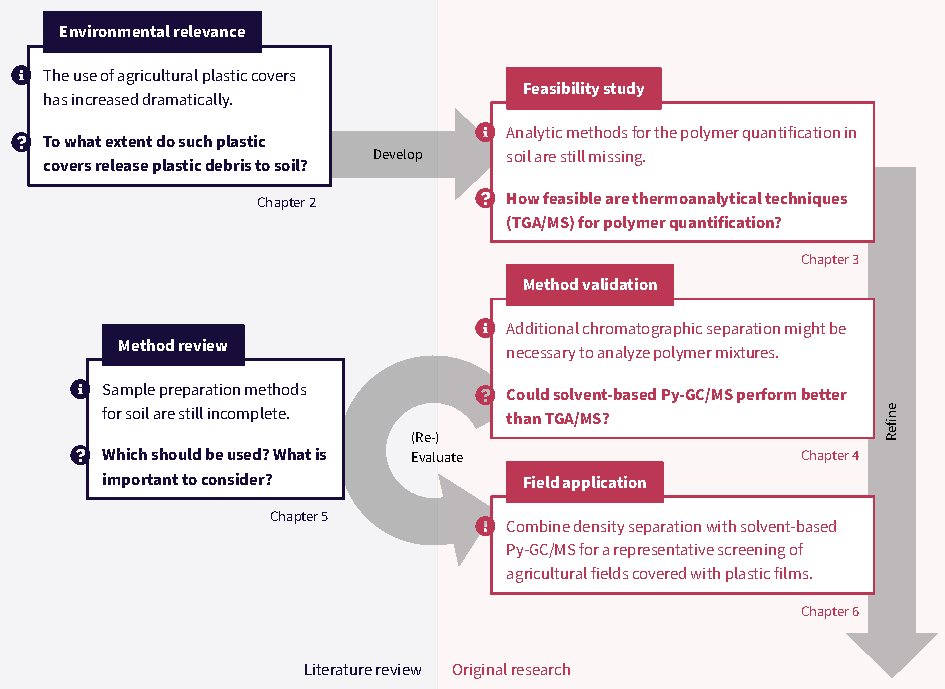
\includegraphics[width=\textwidth]{figures/thesis-overview}
	\caption{Conceptual overview and research questions addressed in this thesis.}
\end{figure*}

Objectives \ref{en:thermoanalysis} to \ref{en:application} were addressed consecutively as each objective relied on the outcome of the previous objective. Objective \ref{en:thermoanalysis} is covered in Chapter~\ref{ch:tga-ms-method}. This first proof-of-principle study used \ac{pet} as a model compound and one reference soil to investigate the potential of \ac{tga-ms} for plastic quantification. The method was designed to enable the rapid analysis of \SI{50}{\milli\gram} soil without any sample preparation. To facilitate the analysis of polymer mixtures and increase instrumental sensitivity, I continued method development using \ac{py-gc-ms} (objective \ref{en:chromatography}). However, \ac{py-gc-ms} is typically restricted to sample amounts \SI{<1}{\milli\gram} which poses high requirements on sample homogeneity. To overcome this and to reduce the risk of potential matrix interferences, I used \acf{tcb} to selectively dissolve \ac{pe}, \ac{pp}, and \ac{ps} in three different reference soils (objective \ref{en:dissolution}). This new solvent-based \ac{py-gc-ms} approach made up to \SI{4}{g} of soil amenable to the quantification of plastic debris (Chapter~\ref{ch:py-gc-ms-method}). Chapter~\ref{ch:analytical-techniques} critically (re-)evaluates this and other analytical techniques. With this knowledge at hand, I further refined my method for its subsequent application (objective~\ref{en:application}, Chapter~\ref{ch:screening}). This involved adjustments in the extraction mixture to increase polymer solubility and the addition of a suitable yet simple sample preparation technique to the existing \ac{py-gc-ms} approach. Thereby, plastic debris could be quantified from \SI{50}{\gram} soil. This sample amount was considered sufficiently large for a representative screening study of eight agricultural fields covered with plastic films (Chapter~\ref{ch:screening}). Therein and in the following discussion (Chapter~\ref{ch:general-discussion}), I conclusively address the key hypothesis of this thesis and reflect on the implications of my findings.
